\chapter{Metallurgy}
\label{chap:metallurgy}
\section{Introduction}
Cottrell observed that metallurgy would require a ``theory... which explains
the properties of metallic solids and the explanation of the origin of this
structure from the structures of individual atoms." Similarly in Vol. 35
Heine noted "What we lack is a fundamental quantum theory of the cohesion
and structure of a wide diversity of solids." The previous chapters,
though hopefully enjoyable in their own right, were really just meant to bring
us to the stage where we can start using the principles of locality
and recursion methods to compute the structural and 
mechanical properties of extended solids.

This chapter will focus on the calculation of the electronic and mechanical
properties of transition metals and their alloys. 

%Perhaps the most interesting aspect of physical metallurgy is how
%macroscopic parameters can be directly connected to the solution of 
%the wave equation governing the atomic scale motion of the electrons.

%Feynman's definition of a chemical bond.
%It now becomes quite clear why the strongest and most important attractive 
%forces arise when there is a concentration of charge between two nuclei. 
%The nuclei on each side of the concentrated charge are each strongly attracted to it.
%Thus they are in effect attracted towards each other. 
%

It is worthwhile reviewing some of the highlights from the history
of first principles calculations of material properties.

The analysis of Wigner and Seitz in many ways initiated the field
of theoretical materials science with their calculation of the cohesive
energy and lattice constant of metallic sodium\cite{wigner33, wigner34}.

Subsequent work in this field extended Wigner and Seitz analysis
to the cohesive and elastic properties of monovalent
metals like sodium, lithium, and copper \cite{fuchs36}. Around
the same time the young quantum theory was being
used to explain the appearance of different phases in alloys in terms 
of Brillouin zones \cite{bethe29, bouckhaert36, owen33, jones34}. 

Born's work provides the standard treatment of 
the stability of lattices to short and long wavelength
vibrations considering general forms for the interatomic potentials\cite{born40,born42},
with other workers again making extensions of the theory to particular
lattice types \cite{power41, nabarro52}. The work of Brockhouse and
others on neutron spectroscopy provided striking experimental confirmation
of many of the predicted properties of lattice vibrations.

In keeping with the unifying theme of the book the targeted quantities
will first be described and formulated in general terms and then mapped
on to a set of recursion calculations to compute the cohesive and elastic
properties of a material from the perspective of the local atomic environment.

\section{Crystal Structure}
Step number uno in the field of theoretical metallurgy is a theory that correctly
describes the crystal structures formed by different pure metals. 
Often the first three lattices encountered by students of metallurgy 
will be FCC, HCP, and BCC.

\begin{quote}
‘Close-packing’ lacks a unique meaning without a specification of 
what is being packed, and what is meant by close and, in particular, 
what is close to what. The thinking underlying the citation of f.c.c. 
and h.p.c. as examples of closest-packed structures is the packing of 
equal hard spheres. A metal is not an assembly of hard spheres,but rather of 
nuclei and electrons.These are both corpundular, with nowhere vanishing 
wavefunctions, but because of their very large mass ratio it is an excellent 
approximation to consider the nuclei as located at points
but the electrons as forming a continuum, with density throughout the metal 
everywhere positive and, except close to the nuclei, quasi-uniform.
\end{quote}

The closeness of close packed structures stems from trying to squeeze
the largest number of atoms into a particular volume
with a hard lower bound on the approach of the Nucleii.
The BCC structure solves a different problem in that it finds a
distribution of nuclei likely to be closest to the electrons.

Early considerations based on orbital hybridisation and geometry
were performed by Altmann, Coulson, and Hume-Rothery who treated 
the problem in Ref.~\cite{altmann57}. One of the earliest triumphs 
of the recursion method was the sorting of the Lave 
Phases \cite{haydocklaves75,johannes76} into distinct structures. 
%Density functional studies of the crystal phases \cite{chan86,paxton97}

The ability of the tight binding framework
to provide an explanatory model for trends in homologous materials is
well demonstrated by the Pettifor's work on the transition
metal series \cite{pettifor70}, the Chevrel compounds of Molybdenum 
chalcogenides Ref.~\cite{bullet77}.
and the structures of the compounds in the Lave phases 
in Ref.~\cite{johannes76},

\section{Lattice Vibrations}
%insight into \cite{varma79a, varma79b}.

\section{Harmonic Approximations to the Free Energy and Entropy}
The crystal structure that is formed at a given temperature is that which
minimizes the Gibbs Free Energy of the system. Most electronic structure calculations
however are done at 0K. A systematic and computationally manageable way of obtaining
finite temperature energies, i.e. free energies is required.

Given a density of states . It is pleasing to report that the recursion method
is ideally suited to computing integrals of exactly that form, rapidly and accurately,
using quadrature methods. Given we now know how to compute electronic and 
vibrational density of states we are in the position to obtain, at no relative additional 
computational cost, vibrational entropies and Free Energies.

The work of Ref.~\cite{wheeler68} combined quadrature approaches
with the calculated moments of vibrational spectra to compute
thermodynamic quantites. For a comprehensive review
of entropic effects in metals and alloys see Ref.~\cite{fultz10}. 
These sources easily equip us with the expressions required. These expressions provide a starting
point for the inclusion of higher order terms in the vibrational spectra
the so called anharmonic effects which can become important at high temperatures.

\section{Stress, Strain, and Elasticity}
Shearing, straining, Young's modulus, poisson ratio, elastic tensors these are the
stuff of every undergraduate materials mechanics course.
Imagine you have some tensor $\epsilon$ and you apply a virtual pure strain to a collection atoms.

The present section will demonstrate how to compute some of the elastic properties
of a BCC crystal using recursion techniques. There are a couple approaches.
One of them involves looking at the changes in the total energy with
respect to a deformation of the lattice and picking out the 
second derivative of this change which, depending on the deformation chosen,
will correspond to an element of the elastic tensor. The second approach
proceeds directly from the Hamiltonian that has been chosen. Second order
perturbation theory allows us to explicitly calculate the contributions of
the Hamiltonian to the elastic constants. The second approach has distinct
numerical and conceptual advantages.

\subsection{The Expressions We Need}
In the author's opinion elasticity is made difficult by the appearance of a variety
of numerical prefactors. An abundance of factors of 2,
1/3, 1/6, etc. seem to arise in the course of a calculation hindering progress. 
We will not attempt to give an introduction to the principles of elasticity rather
we would just provide a collection of equations and some visuals 
that relate deformations of the crystal to changes in total energy.

In this section we shall specialize the analysis to a cubic crystal, specifically a body centered cubic
crystal and simply state the lattice deformations which are required to probe the 
different material elastic constants. We will follow the notation given by Finnis where
a much more detailed exposition can be found along with pointers to comprehensive references.

The first constant we might calculate is the Bulk Modulus which is defined:
%
\begin{equation}
\label{eq:bulkmodulus}
B\equiv V_{c} \frac{\partial^{2} E}{\partial V_{c}^{2}}
\end{equation}
%
that is the second order variation in the energy with respect to changes in the 
sample volume multiplied by the volume. After some rearrangement (which is a useful
exercise) Eq.~\ref{eq:bulkmodulus} can be written:
%
\begin{equation}
V_{c}\frac{\partial^{2} E}{\partial V_{c}^{2}} = \left[-\frac{2}{3}\frac{\partial E}{\partial V_{c}}+\frac{1}{9V_{c}}\frac{\partial^{2}E}{\partial \gamma^{2}} \right],
\end{equation}

where gamma is a scalar that can be varied and controls the change in volume:
%
\begin{equation}
V_{c}(\gamma) = (1+\gamma)^{3}V_{c}(0)
\end{equation}
%

The elastic energy contribution to a sample is written:
%
\begin{equation}
\label{eq:eq:elasticenergy}
E^{elastic} = \frac{1}{2}C_{11}(\epsilon^{2}_{1} + \epsilon^{2}_{2} + \epsilon^{2}_{3}) + C_{12}(\epsilon_{1}\epsilon_{2}
+\epsilon_{2}\epsilon_{3} + \epsilon_{3}\epsilon{1}) + C_{44}(\epsilon^{2}_{4} + \epsilon^{2}_{5} + \epsilon^{2}_{6})
\end{equation}
%
where Voight's notation ($\epsilon_{1}=\epsilon_{xx}$...) has been used. Staring at Eq.~\ref{eq:elasticenergy} you
should be able to see that deformations which pick out only $C_{44}$ or $C_{11}$ should be fairly easy to write down
however $C_{12}$ requires a little more work to pick out on its own.

Let $\epsilon_{ij} = \gamma T_{ij}$, (we like introducing $\gamma$ because it is useful to have a simple scalar
to parametrize the lattice distortions which are written as a matrix $T$).
We can now write the modified lattice constants as:
%
\begin{equation}
R'_{i\alpha} =  R_{i\alpha} + \gamma \sum_{\beta} T_{i\beta}R_{i\beta}
\end{equation}
%

Following Finnis we rewrite Eq.~\ref{q:elastic energy} in terms of the T matrices:

To obtain the shear elastic constant: $C' = \frac{1}{2}(C_{11}-C_{12})$ the following deformation
matrices are particularly helpful a tetragonal distortion:
%
\begin{equation}
T^{t} =  
    \begin{bmatrix}
         1 &   0   & 0  \\
         0 &  -0.5 & 0  \\    
         0 &   0   &-0.5 
    \end{bmatrix}
\end{equation}

or a distortion of the (110) plane:
%
\begin{equation}
T^{(110)} = 
    \begin{bmatrix}
            1 &  0 & 0  \\
            0 & -1 & 0  \\    
            0 &  0 & 0 
    \end{bmatrix}
\end{equation}

To obtain the $C_{44}$ contributions we may introduce
a rhombohedral distortion:
%
\begin{equation}
T^{(111)} =  
    \begin{bmatrix}
             0   & 0.5 & 0.5 \\
             0.5 & 0   & 0.5 \\    
             0.5 & 0.5 & 0 
    \end{bmatrix}
\end{equation}
%
or a (100) distortion:
%
\begin{equation}
T^{(100)} =  
\begin{bmatrix}
             0 & 1 & 0 \\
             1 & 0 & 0 \\    
             0 & 0 & 0 
\end{bmatrix}
\end{equation}
%

For any new potential the computation of the predicted elastic properties should
be the first port of call. For the crystal to be stable $B,C',C_{44}$ must all be
greater than 0 so that gives a definite sanity check on the model. 

Let us apply these deformations to a BCC crystal and see what comes out.

First we'll make a few observations. The deformation matrices for
$C'$ will not change the relative positions of the first nearest neighbours.
This deformation will, however, alter the second nearest neighbour positions so we may expect
that the $C'$ shear will be largely determined by the second nearest neighbour interactions. 
As for the $C_{44}$ distortions all neighbours participate in a rhombohedral distortion
and all neighbours save the two second nearest neighbours orthogonal to the $(100)$
plane participate in a $T^{(100)}$ distortion. 

If we wish to approximate the second derivative of the total energies with 
respect to $\gamma$ we are going to have to be careful. We won't be able
to obtain it by doing a single total energy difference calculation. That
will not contain enough information. We could accomplished it by assuming
an expression of the form: 
\begin{equation}
\Delta E(\epsilon) = 2\epsilon^{2} E^{(2)} + \epsilon^{4} E^{(4)},
\end{equation}
and solving for $E^{(2)}$. Or we could do multiple energy calculations for a sequence 
of distortions and fit a polynomial to the results extracting
the second difference from the polynomial fit.

If you have worked your way through Sec.~\ref{sec:vibrations} you might already have
a set of force constant pairs to hand. In that case Eq.~\ref{eq:brockhouselimit} will give you
another means of obtaining the required elastic constants.
%
\begin{equation}
\label{eq:brockhouselimit}
C_{i} = \frac{1}{B_{i}a}\sum_{n} n^{2}\Phi_{n}
\end{equation}
%
The correspondence between the elastic constant $C_{i}$ and the phonon modes is given
in Table~\ref{tab:brockhouse}:

\begin{table}
\begin{center}
\begin{tabular}{|c|c|}
\hline
Phonon Branch  & Elastic Constant \\
\hline
(00q)L  & $C_{11}$ \\
(00q)T  & $C_{44}$ \\
(qqq)L  & $(C_{11}+2C_{12}+4C_{44})/3$ \\
(qqq)T  & $(C_{11}-C_{12}+C_{44})/3$ \\
(qq0)L  & $C_{11}+2C_{12}+4C_{44}$ \\
(qq0)T1 & ($C_{11}$ - $C_{12}$)/2\\
(qq0)T2 & $C_{44}$\\
\hline
\end{tabular}

\caption{Correspondence of phonon branch with combinations of elastic constants.}
\end{center}
\end{table}

Notice that the factor of $n^{2}$ means you have to be quite confident in the accuracy of
the force constants connecting distant pairs of atoms. Otherwise any error
in your calculation will be rapidly amplified. You should also hope your force
constants are decaying will some alacrity perhaps at least as quickly as $n^{-4}$.

\subsection{Local Stress Fields}
The TBB Model \cite{nielsen83, sutton88} gives us a means of defining and calculating 
a local in the sense of a per atom stress tensor. If $I$ and $J$ 
are cartesian components $x,y,z$ to first order in the energy:
%
\begin{equation}
\delta E^(1) = \sum_{I} \sum_{(ij)}\Omega^{i}\sigma^{i}_{IJ}\epsilon_{IJ}
\end{equation}
%
The contribution to the IJ component of the stress tensor is:
%
\begin{equation}
\label{eq:atomstress}
\sigma^{i}_{IJ} = \frac{1}{\Omega^{i}}\sum_{j\neq i}\sum_{\alpha\beta}G(\epsilon)_{i\alpha j\beta}\frac{\partial H_{j\beta i\alpha}}{\partial R_{jI}}(R_{jJ}-R_{iJ})
\end{equation}
%
The pair contributions can be added to obtain the full stress tensor. 
But if we are only interested in the electronic contributions
Eq.~\ref{eq:atomstress} is already good enough. For an application of the 
see Ref.~\cite{ohta90}

%As usual we need to know the $R$ dependence of our
%integrals, both hopping and on-site, which we went to the trouble 
%of learning in Chapter~\ref{chap:wannier}.

%Ref.~\cite{terakura84} demonstrates how the recursion method
%may be used to compute the elastic constants of a material.

The interaction of dislocations and defects reveals one of the most difficult problems
in theoretical materials science: the coupling of long range elastic fields
with local chemical changes. This coupling of length scales makes
reliable quantitative calculations difficult. Variations in the electronic structure
inducing strains in the metal matrix which feed back into the electronic structure. 
It appears that one requires a theory with quantum accuracy on the scale of an 
interatomic bond that simultaneously takes into account the long range elastic 
field.

%To proceed we will assume we can obtain a relaxed structure where all the atomic forces are
%in equilibrium. We then follow the derivation of Ref.~\cite{freedman09} which uses the free energy
%of the system at equilibrium to derive a tensor that describes the interaction of point defects 
%with elastic fields. A few different ways of computing this tensor are then described \cite{nazarov16}.
%The force method of computing the elastic dipole tensor lends itself 
%immediately to the expressions introduced all the way back in 
%Chapter~\ref{chap:invariance}, Eq.\ref{eq:tbforce}. \cite{paxton90}.

\section{Recursing through Defects and Dislocations}
The ability of the recursion method to quantify the local changes in interatomic bonding and
forces makes it a particularly useful tool for the study of dislocations. 

Understanding the interaction of interstitials and impurities with the motion of
dislocations through a crystal is a central goal of theoretical metallurgy with
with work on this subject beginning in the 1950s \cite{cochardt55}.

The local density of states for atoms at a screw dislocation core have been computed by \cite{paidar81,masuda81}. 
The change in the local bonding picture induced by a vacancy in Fe was examined in Ref.~\cite{masuda82,ohta87}.

\subsection{Charles Frank}
By way of introduction to the variety of dislocation structures that occur
we turn to F.C. Frank. Of Frank-Read dislocations fame.
%Frank wrote a number of interesting article BCC as a 
%close packed structure \cite{frank92}.

\section{Grain Boundaries}
The analysis of Read and Shockley in Ref.~\cite{read50} serves as a comprehensive
introduction to the field of interfaces in condensed matter. The 
standard reference on the subject of interfaces in materials is Sutton and 
Baluffi Ref.~\cite{sutton95}.

A number of experimental probes are capable of detecting the presence of 
grain boundaries but efficient and accurate means of determining 
the orientation relationships between grains remains an outstanding problem.
For an analysis of the statistic arrangement of grains using quaternion
algebra see Ref.~\cite{sutton96}.
%structural unit model sutton 89
The possibility of examining grain boundaries atomistically has interested
researchers since it became practical to perform atomistic simulations
with realistic potentials see Refs.~\cite{bristowe75,wolf83,paxton87,paxton88,paxtonsutton88,
kohyama88,kohyama94,paxton96,rittner96,tschopp07,momida13,du11,du12,mceniry18} for a
snapshot of the way computational studies of interfacial structure 
has evolved over time.

There is incredible scope for behaviour at the boundarys.

\subsection{Discrete Boundary Dislocation Networks}
Combining isotropic elasticity with discrete dislocation networks
we can gain some useful practice in contour integration and arrive
at a closed set of expressions for strains in linear elasticity
theory next to a large angle grain boundary. 

These expressions are given in Ref.~\cite{sutton95} and derived here.

\subsubsection{Grain Boundary Algebra}
\label{gbalgebra}
%Just for reference, the algebra is similar for all other components of the stress, and
%can be extended to cases where we have a traveling edge dislocation i.e. instead of
%a sum over n $n$ we have a factor like (y-vt)....
First we introduce the function:
%
\begin{equation}
f(z) =  \pi\cot(\pi z)\frac{(Y-z)(3x^{2} + (Y-z)^{2})}{(X^{2} + (Y-z)^{2})^{2}}
\end{equation}
%
This has simple poles at $z = 0, \pm 1, \pm 2,...$. It also has two 2nd 
order poles at  $z_{1}=iX+Y$, $z_{2}=-iX+Y$. The residue at $z_{2}$ can
be found from the following expression: 
%
\begin{equation}
{\rm Res}(z_{2}) = \lim_{z\rightarrow z_{2}}\frac{d}{dz}(z-z_{2})^{2}
\frac{\cot(\pi z)(Y-z)(3X^{2}+(Y-z)^2)}{(z-z_{1})^{2}(z-z_{2})^{2}}
\end{equation}


\begin{align}
\label{eq:2ndstep}
{\rm Res}(z_{2})&=\frac{\pi^{2}}{\sin^{2}(\pi z_{2})}\left[\frac{(Y-z_{2})(3x^{2}+(Y-z_{2})^{2})}{(z_{2}-z_{1})^{2}}\right]\\
  &+\frac{\pi\cot(\pi z_{2})}{(z_{2}-z_{1})^{2}}\left[-(3x^{2} + (Y-z_{2})^{2})-2(Y-z_{2})^{2}\right] \\
  &+\frac{2\pi\cot(\pi z)(Y-z_{2})(3X^{2}+(Y-z_{2})^{2})}{(z_{2} - z_{1})^{3}}
\end{align}
%
The second term in Eq.~\ref{eq:2ndstep} evaluates to zero and the remaining terms can be simplified to:
%
\begin{equation}
{\rm Res}(z_{2}) = \frac{\pi}{4\sin^{2}(\pi(Y-iX))}(i\pi X - \sin(2\pi(Y-iX)))
\end{equation}
%
The residue at $z_{1}$ can be found in a similar manner.

If we construct a set of contours as depicted in Fig.~\ref{fig:polediagram}.
\begin{figure}[!tbp]
\begin{center}
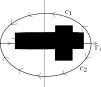
\includegraphics[scale=1.0]{stresspolediagram.pdf}
\caption{Contours to determine sum. The lines of poles from the $\cot(\pi z)$ 
factor can be equated to the difference of the two 
second order residues.\label{fig:polediagram}}
\end{center}
\end{figure}


We can write down the sum as the difference of the two second order residues.

\subsubsection{Jordan's lemma}
We must consider the behaviour of the function $f(z)$ on the countours carefully in order to determine their contribution to the $\oint f(z) dz$ as we expand the semi-circular contours out to $\infty$.  Jordan's lemma says if we are able to write $f(z) = \exp(iaz)g(z)$ for positive $a$ then an upper-bound for the integral over the semi-circular contour in the upper-half plane is given by
\begin{equation}
\left|\int_{C_{1}}f(z)dz\right| \leq \frac{\pi}{|a|}\text{max}_{\theta\in [0,\pi]}\left|g(Re^{i\theta})\right|
\end{equation}
A similar results holds for the lower-half plane, provided we now make $a<0$.  We now consider expansions for $\cot(\pi z)$:
\begin{eqnarray}
\cot(\pi z)&=&-i(e^{i2\pi z}+1)(1-e^{i2\pi z})^{-1}=-i(1+e^{i2\pi z})(1+e^{i2\pi z}+e^{i4\pi z}+\ldots)\label{eq:upper}\\
&=&i(1+e^{-i2\pi z})(1-e^{-i2\pi z})^{-1}=i(1+e^{-i2\pi z})(1+e^{-i2\pi z}+e^{-i4\pi z}+\ldots)\label{eq:lower}
\end{eqnarray}
Focusing first on the upper-half plane we replace $\cot(\pi z)$ with equation~\ref{eq:upper}.  Since $g(z)=f(z)/\cot(\pi z)$ goes to zero as $z\rightarrow\infty$ we can apply Jordan's lemma and ignore the contributions on $C_{1}$ from all positive powers of $e^{i2\pi z}$.  However we still need to consider the $-i$ term, where Jordan's lemma doesn't apply.  Substituting $z=Re^{i\theta}$ and taking the limit as $R\rightarrow\infty$ we obtain:
\begin{equation}
\int_{C_{1}}f(z)dz = \int_{\theta=0}^{\pi}d\theta iRe^{i\theta}*\frac{(i\pi R^{3}e^{3i\theta}}{R^{4}e^{4i\theta}} = -\pi^{2}
\end{equation}
We now instead focus on $C_{2}$ and replace $\cot(\pi z)$ with equation~\ref{eq:lower}.  Once again Jordan's lemma allows us to ignore the powers of $e^{-i2\pi z}$.  However we still need to focus on the $i$ term.  Substituting $z=Re^{i\theta}$ and taking the limit as $R\rightarrow\infty$ we obtain:
\begin{equation}
\int_{C_{2}}f(z)dz = \int_{\theta=2\pi}^{\pi}d\theta iRe^{i\theta}\times\frac{(-i\pi R^{3}e^{3i\theta})}{R^{4}e^{4i\theta}} = -\pi^{2}
\end{equation}

Let $I=\int_{\Gamma_{1}}f(z)dz$, then closing on the upper-half plane we have:
\begin{equation}
I-\pi^{2} = 2\pi i\left[Res(z_{1})+\sum_{n=-\infty}^{\infty}Res(z=n)\right]
\end{equation}
While closing on the lower-half plane gives:
\begin{equation}
I-\pi^{2} = -2\pi i Res(z_{2})
\end{equation}
(note, negative sign is since the contour goes clockwise on the lower-half plane).

\subsection{Dislocation-Interstitial Interactions}
Coupling of the hydrogen defects to the screw and edge dislocations can be
handled via the approach taken in \cite{cochardt55}.
The interaction energy between a dislocation and an interstial atom can
be calculated from the work done by moving each face of a cell a distance
$d_{i}$ against a force $F_{i}$ exerted by the stress field:
%
\begin{equation}
U_{DC} =+\sum_{i}F_{i}d_{i}
\end{equation}
%
If the components of the stress tensor are assumed constant along the distance $a$
this energy can be written:
%
\begin{equation}
U_{\rm{DC}} = -(T_{D},S_{H})a^{3}= -\sum_{ik} \sigma_{ik}^{D}\epsilon^{H}_{ik} a^{3}
\end{equation}
%

The observed slip system in $\alpha$-Fe for a screw dislotion is along the [111]
direction. Away from the dislocation core a bulk cell can be found and defined
with three unit vectors [100], [010], [001]. This unit cell is drawn in
Fig.~\ref{fig:interstitialcoords} (a). For an edge dislocation the slip plane is
assumed to be in the $(0\bar{1}1)$-plane, the dislocation line is in the direction
$\langle 211 \rangle$, and a Burgers vector in the direction $\langle \bar{1}11 \rangle$.

\begin{figure}[!tbp]
\begin{center}
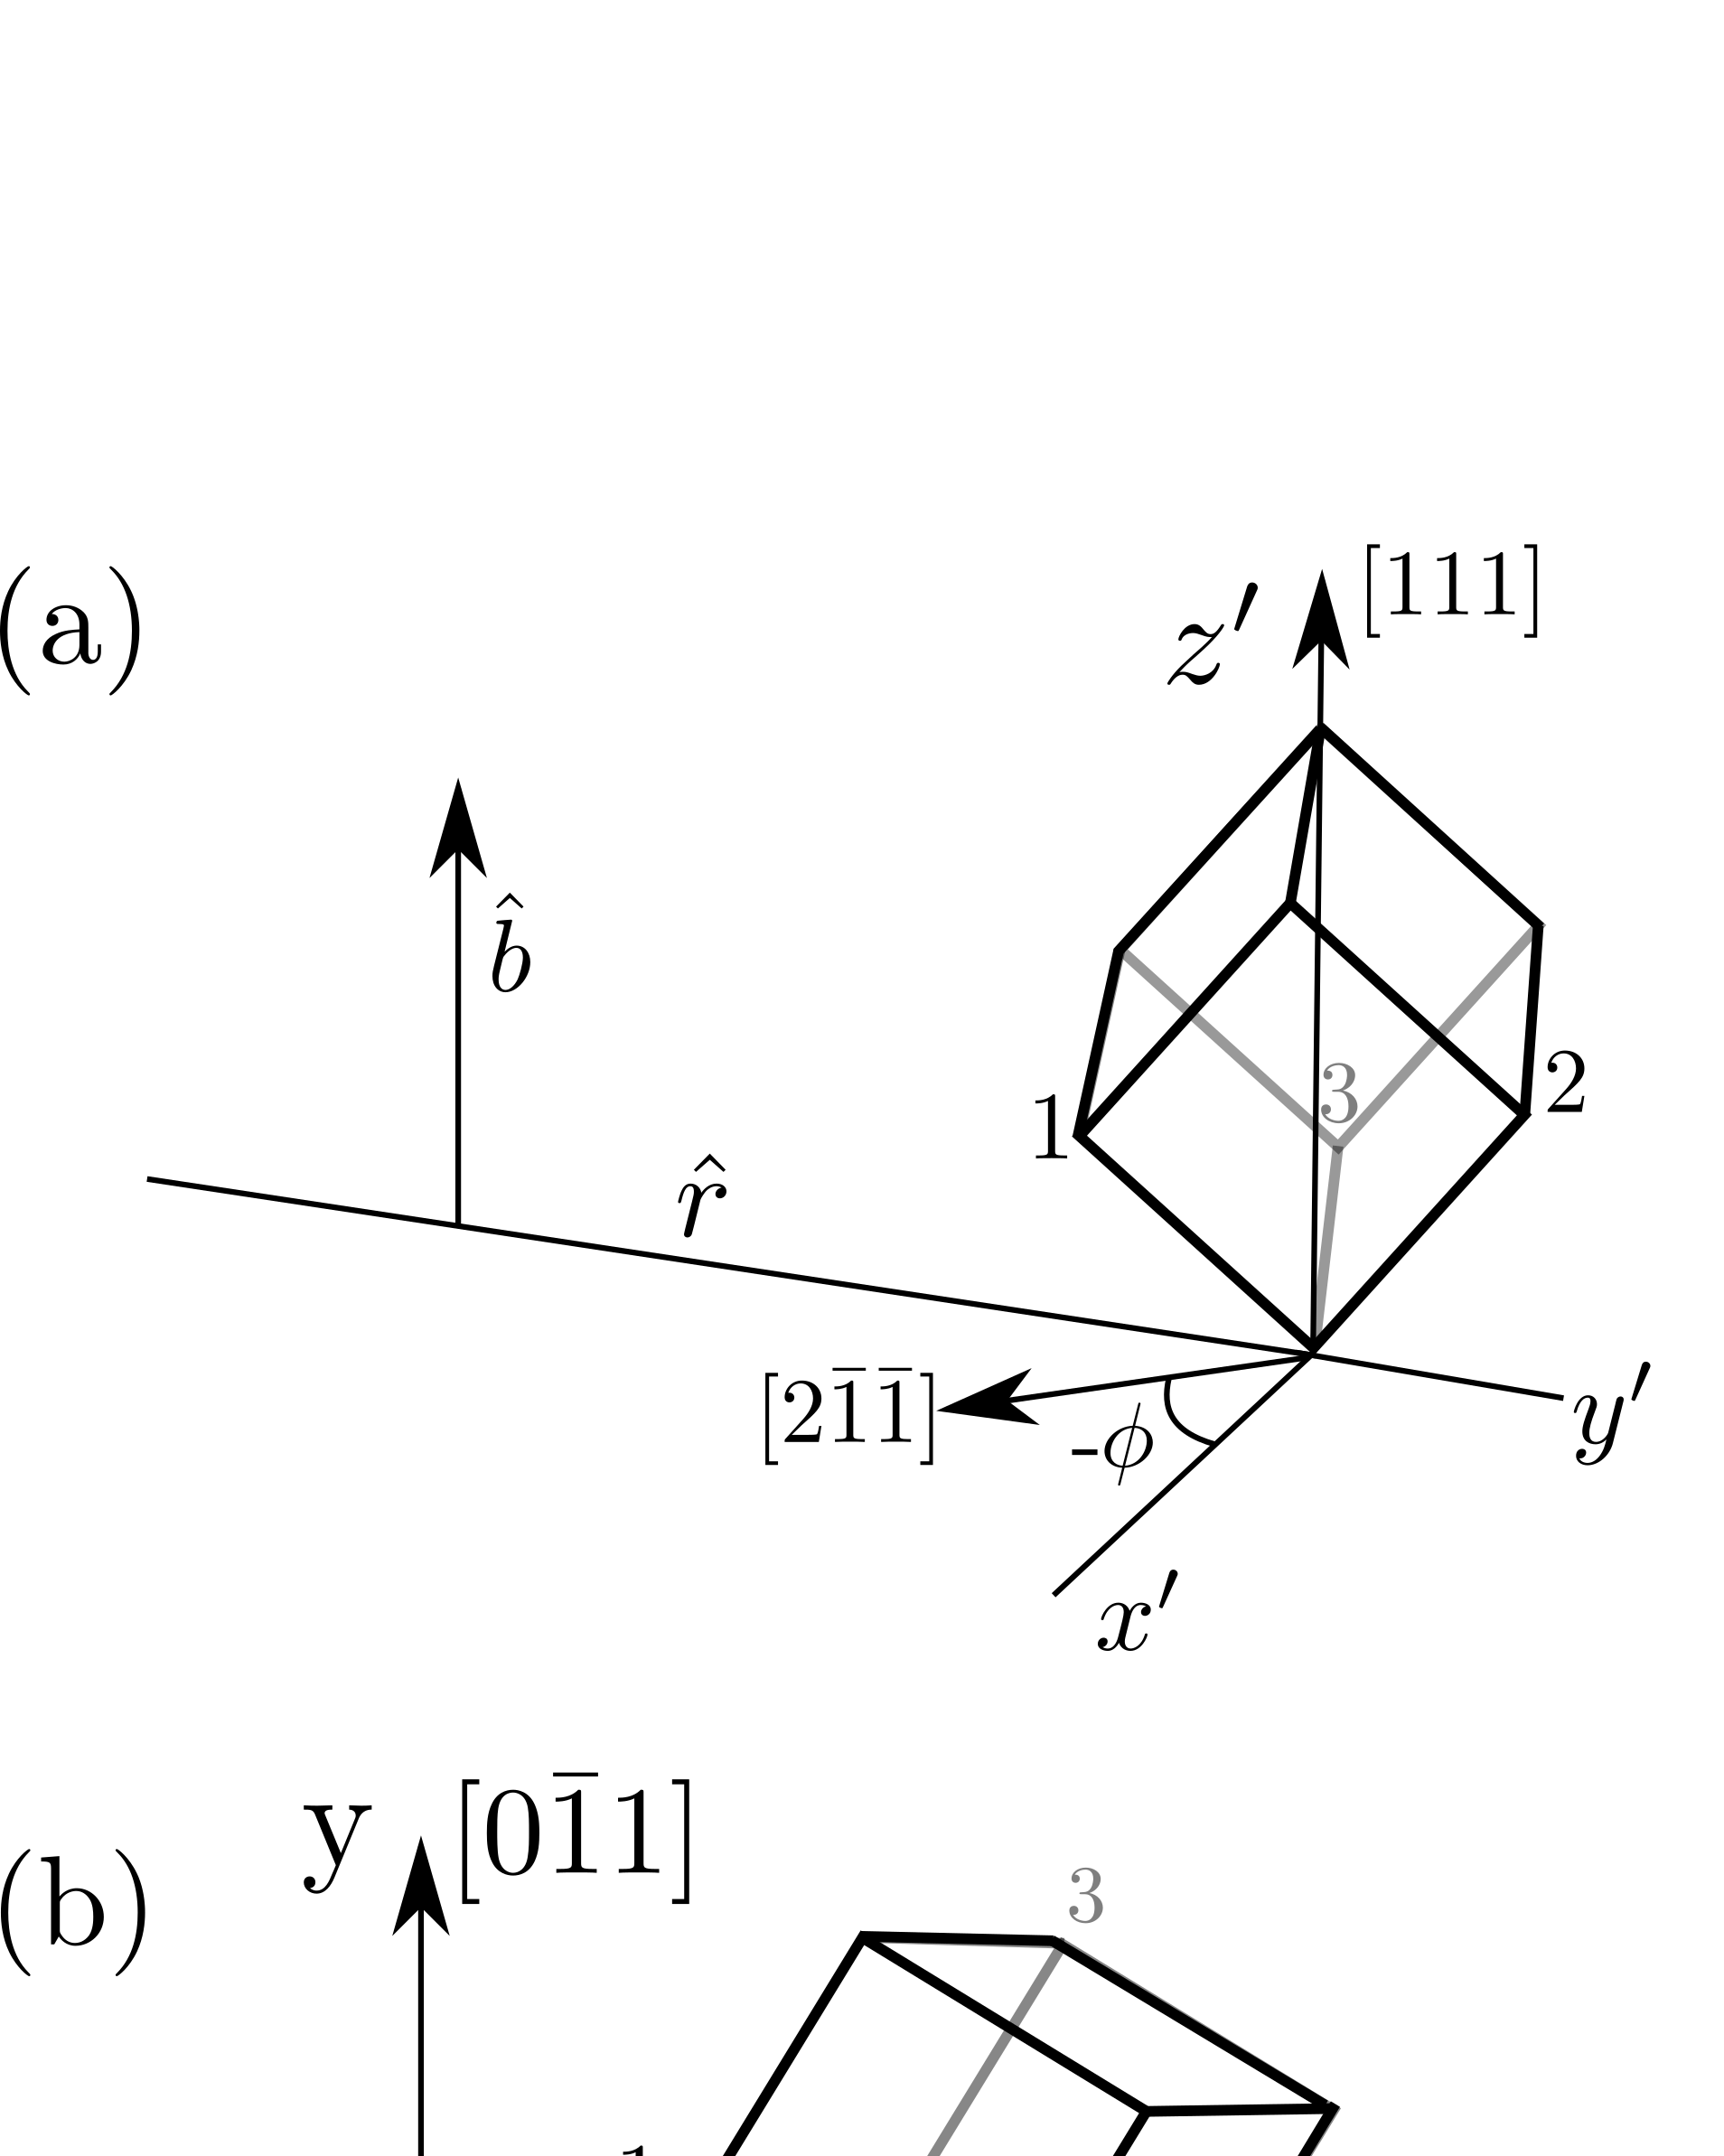
\includegraphics[scale=0.8]{screwcoordinate.png}
\caption{\label{fig:interstitialcoords} Reproduced from \cite{cochardt55}.}
\end{center}
\end{figure}
%
In the analysis of Cochardt they calculate the interstitial-dislocation
energy for the defect atom, Carbon, at a distance $b$. In each case we
wish to translate the defect strain tensor into the

This can be accomplished by determining the transformation matrix $\mathbf{R}$:
which is the inverse of the matrix constructed by stacking up
the basis vectors in the new coordinate system,
%
\begin{equation}
\epsilon'_{ij} = \mathbf{R} \epsilon_{ij} \mathbf{R}^{\rm T}
\end{equation}
%
In \cite{cochardt55} the strain tensor for a carbon atom in
a conventional rectangular unit cell for BCC iron is:
%
\begin{equation}
\left(
\begin{array}{ccc}
 a & 0 & 0 \\
 0 & b & 0 \\
 0 & 0 & c  \\
\end{array}
\right),
\end{equation}
%

The stress tensor in the vicinity of a screw dislocation:
%
\begin{equation}
T^{x',y',z'}_{D}=
\frac{Gb}{2\pi r}
\left(
\begin{array}{ccc}
0 & 0 & 1 \\
0 & 0 & 0 \\
1 & 0 & 0 \\
\end{array}
\right)
\end{equation}
%
and the stress tensor in the vicinity of an edge dislocation:
\begin{equation}
T^{x',y',z'}_{D}=
\frac{Gb}{2\pi(1-\nu)r}
\left(
\begin{array}{ccc}
-\sin\psi(1+2 \cos^{2}\psi) & \cos\psi\cos 2\psi & 0 \\
\cos\psi\cos 2\psi & \sin\psi\cos 2\psi & 0 \\
0 & 0 & -2\nu\sin\psi \\
\end{array}
\right)
\end{equation}
%
where the components of the tensor are estimated from X-ray measurements
of the tetragonal distortion of martensite to be $\epsilon_{a}=0.38$,
$\epsilon_{b}$=$\epsilon_{c}$=-0.026. For the screw dislocation
geometry given in Fig.~\ref{fig:interstitialcoords} (a) the transformed strain
tensor is:
%
%
\begin{equation}
\mathbf{\epsilon}'=\left(
\begin{array}{ccc}
 \frac{1}{3}[a+2 b+(a-b) \cos (2 \theta)] & -\frac{1}{3} (a-b) \sin (2 \theta ) & \frac{\sqrt{2}}{3} (a-b)\cos(\theta )\\
 -\frac{1}{3} (a-b) \sin (2 \theta ) & \frac{1}{3} (a+2 b+(b-a) \cos (2 \theta )) & -\frac{\sqrt{2}}{3}(a-b) \sin (\theta )\\
 \frac{\sqrt{2}}{3} (a-b) \cos (\theta ) & -\frac{\sqrt{2}}{3}(a-b)\sin(\theta ) & \frac{1}{3}(a+2 b)\\
\end{array}
\right).
\end{equation}
%
For the edge dislocation the inner product of the basis vectors does not vary with $\theta$
and the transformed strain tensor is given as:
%
\begin{equation}
\mathbf{\epsilon}'=\left(
\begin{array}{ccc}
 \frac{1}{3} (a+b+c) & \frac{c-b}{\sqrt{6}} & \frac{-2 a+b+c}{3 \sqrt{2}} \\
 \frac{c-b}{\sqrt{6}} & \frac{b+c}{2} & \frac{c-b}{2 \sqrt{3}} \\
 \frac{-2 a+b+c}{3 \sqrt{2}} & \frac{c-b}{2 \sqrt{3}} & \frac{2}{3}a + \frac{1}{6}(b+c) \\
\end{array}
\right).
\end{equation}

\subsection{Pile Ups}
Another interesting case is discussed in Ref.~\cite{eshelby} 
where free dislocations pile up next to a pinned dislocation.

\section{Alloys}
The application of the recursion method to random lattices is described.
\cite{glaser81}
%
\begin{equation}
H_{nm} = e_{n}\delta_{nm} + V_{nm}
\end{equation}
%
Mookerjee and Haydock extended the recursion method to the case of random alloys.
The developement of the recursion method to handle random material systems is 
itself quite ingenious \cite{mookerjee, haydock74}. The Hamiltonian is extended
so that tight binding hops on a real lattice are made along with potential hops
on a "field" lattice. The field lattice can be cast in tridiagonal form to represent
the underlying statistical distribution of the random alloy. Different graphs are available
to represent rectangular random distributions, binary distributions, Gaussian distributions
etc. Fig.~\ref{fig:fieldsite.png} gives an example of the first few hops on a "field-site" 
lattice to obtain the averaged value of a Green's function. The hopping of the recursion method
is now coupling lattice sites and taking into account the underlying distribution of 
the underlying parameters.

Despite its elegance the number of paths now emanating from an initial orbital, both
for electrons to hop from orbital to orbital (lattice hops) and for the hops between 
statistical configurations (field hops) are considerable and simplifying approximations 
need to be found due to the difficulty of enumerating all the possible paths.

Early work on DOS of alloys \cite{cubiotti77}. 

\section{Metallic Surfaces}
Elegant experimentation can access some surprisingly delicate quantities \cite{whipp34}.
See \cite{bullet77} for calculations of the adsorption energy of H on W and Pt.

\section{Conclusion}
In this chapter we have looked at a number of the important quantities that
arise in metallurgy and how the recursion method is ideally suited to their 
computation. The motion of dislocations, the structure of grain boundaries, 
and alloying. 

%Masuda-Jindo ISIJ 28, 843 (1988)
%Dilute Alloys
%J Friedel Adv. Phys. 3, 446 (1954)
%Non-Hermitian Matrices
%R. Haydock and M.J. Kelly. J. PHys. C 8, L290
%R. Haydock, J. Phys. A 7, 2120 (1974)
%Lave Phases:
%A. K. Sinha, Prog. Mater. Sci. 15, 81 (1972)
%Anderson Localization
%R. Haydock Philos. Mag. [Part] B 37, 97 (1978)
%R. Haydock and A. Mookerejee, J. Phys. C 7, 3001 (1974)
%UV Photoemission
%R. K. C. McLean and R. Haydock, J. Phys. C 10, 1929 (1977)
%https://materialscience.uoregon.edu/wp-content/uploads/2016/02/tightbind.pdf
%Self-Consistent Tight Binding Orbitals
%Philos. Mag [8] 35, 845 (1977) #
%Binary Alloys 
%R. L. Jacobs, J. Phys. F 3, 933 (1973)
%and stacking in La \cite{duthie77}.
%Atomic stress tensors:
%Sutton 88
%Nielsen O H and Martin R M 1983 Phys. Rev. Lett. 50 697
%Nielsen O H and Martin R M 1985a Phys. Rev. B 32 3780
%-                          1985b Phys. Rev. B 32 3792
